\documentclass[a4paper, 12pt]{article}
\usepackage[top=2cm, bottom=2cm, left=2.2cm, right=2.2cm]{geometry}
\usepackage[utf8]{inputenc}
\usepackage{amsmath, amsfonts, amssymb}
\usepackage{amsthm}
\usepackage{indentfirst}
\usepackage{graphicx}
\usepackage{gensymb}
\usepackage{float}
\title{Universidade de São Paulo \\ EESC}
\author{SEM0530 - Problemas de Engenharia Mecatrônica II \\ 
Prof. Marcelo Areias Trindade \\ \\ Prática 2 - Aproximação de integrais
\\ \\ Aluno: Marcus Vinícius Costa Reis (12549384)}
\date{08/06/2022}

\begin{document}
	\maketitle \newpage \tableofcontents \newpage
	
	\section{Problema}
	
	Um veículo se desloca com trajetória circular de raio $r=100\,m$. Considerando que ele inicia o movimento com velocidade 
	inicial de $v_0=(10+0.1N)\,m/s$ e acelera com $a_t=(4-0.01s^2)\,m/s^2$ (onde $N=84\Rightarrow v_0=18.4\,m/s$):
	
	\begin{itemize}
		\item Determine o módulo da velocidade do veículo desenvolvida ao longo da trajetória $v(s)$, faça um gráfico 
		($v$ vs $s$), e calcule a velocidade alcançada depois de percorrer $20\,m$.
		\item Determine o módulo da aceleração do veículo ao longo da trajetória $a(s)$, faça um gráfico ($a$ vs $s$), e 
		calcule a aceleração alcançada depois de percorrer $20\,m$.
		\item Usando um método numérico de aproximação de integrais, determine o tempo necessário para o veículo 
		percorrer $20\,m$.
	\end{itemize}
	
	\section{Formulações}
	
	Em primeira instância, tendo em vista a dinâmica do problema em questão, vale relembrar alguns princípios da cinemática
	escalar, os quais auxiliarão nas determinações requeridas.
	
	Tem-se que o módulo da velocidade $v$ de um ponto material em uma dada trajetória correponde à taxa de variação da 
	posição $s$ em função do tempo $t$: \begin{equation} v=\dfrac{ds}{dt}	
	\end{equation}
	
	A seu turno, o módulo da aceleração tangencial $a_t$, responsável por alterar o módulo de $v$, é dada por: 
	\begin{equation} 
		a_t=\dfrac{dv}{dt}
	\end{equation}				
	
	Comparando as eq. 1 e 2:
	$$\dfrac{1}{v}\,ds=\dfrac{1}{a_t}\,dv \Longleftrightarrow a_t\,ds=v\,dv$$ 
	\begin{equation}
		\Longleftrightarrow \int a_t(s)\,ds=\int v\,dv
	\end{equation}		
	
	Desse modo, se a aceleração tangencial é conhecida como função da posição, consegue-se encontrar $v$ em função de $s$.
	
	Da eq. 1 ainda é possível obter: $$dt=\dfrac{1}{v}\,ds\Longleftrightarrow$$
	\begin{equation}
		\int dt=\int \dfrac{1}{v(s)}\,ds
	\end{equation}
	
	Portanto, de forma análoga, obtém-se o tempo em função da posição se é conhecida a expressão de $v$ em função de $s$.
	
	Vale ainda ressaltar que o problema em questão anlisa um movimento circular. Sendo assim, há também uma componente normal
	$a_n$ da aceleração, a qual é dada por:
	\begin{equation}
		a_n=\dfrac{v^2}{r}
	\end{equation}
	
	\newpage
	
	O módulo da aceleração do ponto material é, por conseguinte, composição das duas componentes:
	\begin{equation}
		a=\sqrt{a_t^2+a_n^2}
	\end{equation}
	
	Pode-se, agora, partir para as determinações desejadas.	
	
	\section{Resultados}
	
	\subsection{Velocidade}
	
	Utilizando-se a eq. 3, juntamente com as informações $a_t(s)=(4-0.01s^2)\,m/s^2$ e $v_0=18.4\,m/s$, obteve-se:
	
	$$\int_0^s (4-0.01s^2)\,ds=\int_{18.4}^{v(s)} v\,dv$$
	$$\Longrightarrow \left[\frac{1}{2}v^2\right]_{18.4}^{v(s)}=\left[4s-\frac{0.01}{3}s^3\right]_{0}^{s}
	\Longrightarrow v^2(s)=8s-\frac{0.02}{3}s^3+18.4^2$$
	\begin{equation}
		\Longleftrightarrow v(s)=\sqrt{338.56+8s-\frac{0.02}{3}s^3}\,\,\,\,(m/s)
	\end{equation}
	
	Avaliando a expressão anterior em $s=20\,m$: $$v_{20}=v(20)=21.1\,m/s$$
	
	\subsection{Aceleração}
	
	Com a eq. 5 e o dado $r=100\,m$, pôde-se encontrar a expressão para a aceleração normal:
	\begin{equation}
		a_n(s)=\frac{v^2(s)}{r}=\frac{1}{100}\left(338.56+8s-\frac{0.02}{3}s^3\right)\,\,\,\,(m/s^2)
	\end{equation}
	
	Utilizando-se da eq. 6 e da expressão dada para $a_t(s)$, chegou-se ao módulo da aceleração da partícula:
	$$a(s)=\sqrt{a_t^2(s)+a_n^2(s)}\Longrightarrow a(s)= \sqrt{(4-0.01s^2)^2+
	\left[\frac{1}{100}\left(338.56+8s-\frac{0.02}{3}s^3\right)\right]^2}$$
	$$\Longleftrightarrow a(s)=1.5\times 10^4[s^6+(2.01\times 10^4)s^4+(-1.01568\times 10^5)s^3+(-1.656\times 10^7)s^2+$$
	$$+\,(1.21882\times 10^8)s+6.17901\times 10^9]\,\,\,\,(m/s^2)$$
	
	Avaliando a expressão anterior em $s=20\,m$: $$a_{20}=a(20)=4.4523\,m/s^2$$
	
	\subsection{Tempo}
	
	Por meio da eq. 4, bem como da expressão 7, chegou-se à relação para o tempo $t_{20}$ decorrido após a partícula ter
	percorrido $20\,m$: $$t_{20}=\int_{0}^{t_{20}}\,dt=\int_{0}^{20}\frac{1}{v(s)}\,ds\Longrightarrow$$
	
	\newpage
	
	$$\Longrightarrow t_{20}=\int_{0}^{20}\frac{1}{\sqrt{338.56+8s-\dfrac{0.02}{3}s^3}}\,ds=
	\int_{0}^{20}\left(338.56+8s-\frac{0.02}{3}s^3\right)^{-\frac{1}{2}}\,ds$$
	
	Como é possível perceber, a integral anterior não é de trivial resolução. Nesse sentido, optou-se pelo emprego de algumas
	ferramentas computacionais proporcionadas pelo software \textit{Octave}, no intuito de aproximar seu resultado por meio
	de métodos numéricos.
	
	Antes, porém, acreditou-se ser pertinente a visualização gráfica da área sob o gráfico da curva relativa ao integrando 
	($1/v(s)$), de modo a possibilitar a obtenção de uma noção sobre o valor procurado. Tal empreitada é mostrada no Gráfico 1.	
	
	\begin{figure}[H]
		\centering
		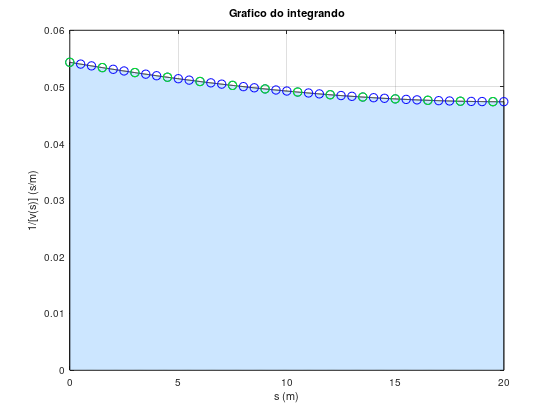
\includegraphics[scale=1]{g3.png}
		\caption{Gráfico 1: Área sob a curva do integrando}
	\end{figure}
	
	Por uma análise meramente visual da área $A$ obtida, pode-se fazer uma primeira aproximação para seu valor. É possível 
	notar que a área em questão pode ser aproximada por um retângulo de base $20$ e altura $0.05$. Haveria uma subestimação 
	aproximadamente no trecho $[0,10]$ e uma superestimação no trecho subsequente $(10,20]$. No entanto, visualmente essas
	flutuações parecem se cancelar. Sendo assim, o retângulo mencionado parece uma boa aproximação inicial.
	
	Logo: $$A_{inicial}\approx 20\cdot 0.05=1$$
	
	Mas, a área $A$ representa o tempo $t_{20}$ decorrido. 
	
	Portanto: $$t_{20}\approx 1\,s$$
	
	\newpage
	
	\subsubsection{Função \textit{trapz}}
	
	A princípio, optou-se pela utilização do método \textit{trapz} do \textit{Octave}, que aproxima a área cujo valor 
	se deseja obter por meio de trapézios. O método depende da discretização escolhida. Sendo assim, realizou-se três
	discretizações distintas para fins de comparação de resultados, as quais são mostradas no Gráfico 1, uma em preto,
	outra em círculos azuis, e outra em círculos verdes:
	
	\begin{itemize}
		\item Discretização em \textit{preto}: $s_1=[0:.1/50:20]$
		\item Discretização em \textit{azul}: $s_2=[0:.5:20]$
		\item Discretização em \textit{verde}: $s_3=[0:1.5:20]$
	\end{itemize}
	
	Desse modo, aplicando as discretizações ao método \textit{trapz}, chegou-se aos valores de $t_{20}^i$ respectivos às
	discretizações $s_i$, $i=1,2,3$ : $$t_{20}^3=0.9725\,s\,,\,\,\,t_{20}^2=0.9961\,s\,,\,\,\,t_{20}^1=0.9961\,s$$
	
	O comando utilizado no prompt do \textit{Octave} foi $t_{20}^i=$ \textit{trapz}($s_i,y_i$), onde $y_i=1/v(s_i)$,
	para cada $i=1,2,3$.
	
	Obviamente, as variáveis foram declaradas de modo a estar de acordo com a sintaxe do software.
	
	Analisando os resultados, vê-se que, para a precisão escolhida, os valores de $t_{20}^2$ e $t_{20}^1$ foram idênticos,
	apontando para a convergência para o valor apresentado. Mesmo a discretização mais grossa, $s_3$, não produziu um 
	resultado discrepante; pelo contrário, foi bem próximo ao das outras discretizações mais finas.
	
	Essa proximidade de resultados pode ser justificada pela suavidade da curva acima da área calculada, como constatado no
	Gráfico 1. Outrossim, a aproximação inicial $t_{20}\approx 1$ chegou muito próxima de $0.9961$.	
	 
	\subsubsection{Função \textit{quad}}
	
	No intuito de obter uma comparação entre os métodos, além de ter outra via para a obtenção do valor de $t_{20}$,
	optou-se por utilizar, também, o método \textit{quad} do \textit{Octave}. Tal método se utiliza da regra de Simpson para
	aproximar o valor da integral com uma precisão de $10^{-6}$ por \textit{default}.
	
	Optou-se por realizar o comando no prompt do \textit{Octave} e utilizar a declaração de uma \textit{anonymous function}. 
	As linhas de código utilizadas foram as seguintes:	
	
	\begin{itemize}
		 \item $>>$ integ = @$(s)\,\,\,(-(0.02/3)*s.\^\ 3+8*s+338.56).\^\ (-1/2);$		 
		 \item $>>$ \textit{quad}(integ, $0$, $20$)
	\end{itemize}
	
	O retorno foi \textit{ans} $=0.9961$. Assim: $$t_{20}^{quad}=0.9961\,s$$
	
	\newpage
	
	\subsubsection{Algumas breves comparações}
	
	No intuito de comparar o resultado mais preciso dentre os obtidos pelo uso da \textit{trapz}, $t_{20}^1$ e o valor 
	$t_{20}^{quad}$ obtido a partir da função \textit{quad}, formatou-se os mesmos com o comando \textit{format long}.	
	
	Obteve-se: $$t_{20}^1=0.996082859579149\,,\,\,\,t_{20}^{quad}=0.996082859365112$$
	
	Calculando a diferença relativa entre eles: $$\frac{|t_{20}^{quad}-t_{20}^1|}{|t_{20}^{quad}|}\cdot 100\approx 
	2\times 10^{-8}\,\%$$
	
	Pela ínfima diferença, é válido assumir o valor $$t_{20}=0.99608286\,s$$ como a solução para o problema.
	
	Pode-se, agora, verficar o erro da aproximação visual inicial: $$\frac{|t_{20}-t_{20}^{aprox}|}{|t_{20}|}\cdot 100
	\approx 4\times 10^{-1}\,\%$$
	
	É possível dizer, então, que, nesse caso, a aproximação visual foi bastante confiável.
	
	\section{Gráficos}
	
	Nessa seção, são apresentados os gráficos da velocidade e da aceleração desenvolvida pela partícula.
	
	Algo interessante a ser notado é que $v_{20}$ corresponde ao máximo de velocidade no trecho analisado, o que pode ser
	comprovado quando se observa $$\frac{dv(s)}{dt}=a_t(s)=4-0.01s^2=0\Longleftrightarrow s=\pm \sqrt{400}=\pm 20\,m$$
	
	A seu turno, $a_{20}$ corresponde a um mínimo de aceleração, já que $a_t(20)=0$, e, portanto, a contribuição para o
	módulo de $a(s)$ provém unicamente de $a_n(s)$.
	
	\begin{figure}[H]
		\centering
		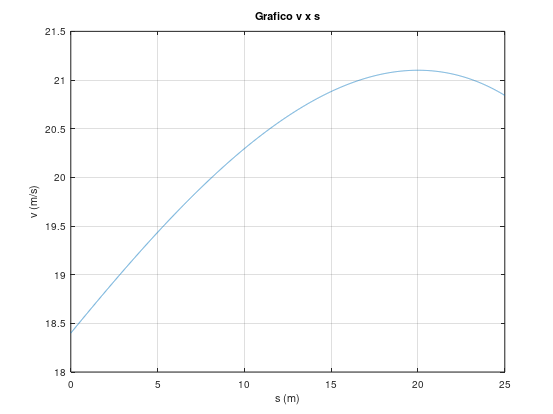
\includegraphics[scale=1]{g1.png}
		\caption{Gráfico 2: curva da velocidade $v(s)$}
	\end{figure}
	
	\begin{figure}[H]
		\centering
		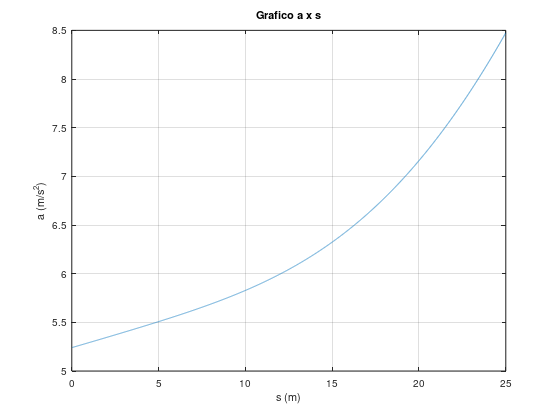
\includegraphics[scale=1]{g2.png}
		\caption{Gráfico 3: curva da aceleração $a(s)$}
	\end{figure}
	
	\newpage
	
	\section{Scripts}
	
	A seguir, encontram-se os scripts em \textit{Octave} utilizados para a construção dos gráficos e para o cálculo dos 
	valores da velocidade e da aceleração na posição $s=20\,m$.
	
	\begin{figure}[H]
		\centering
		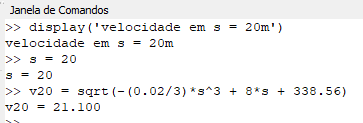
\includegraphics[scale=1]{img1.png}
		\caption{Cálculo de $v_{20}$}
	\end{figure}
	
	\begin{figure}[H]
		\centering
		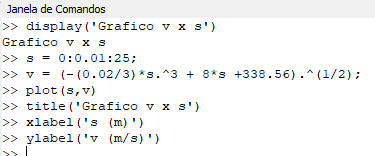
\includegraphics[scale=1]{img2.png}
		\caption{Construção do Gráfico 2}
	\end{figure}
	
	\begin{figure}[H]
		\centering
		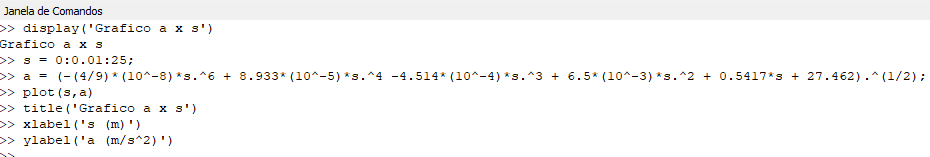
\includegraphics[scale=1]{img3.png}
		\caption{Construção do Gráfico 3}
	\end{figure}
	
	\begin{figure}[H]
		\centering
		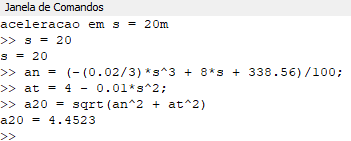
\includegraphics[scale=1]{img4.png}
		\caption{Cálculo de $a_{20}$}
	\end{figure}
	
	\begin{figure}[H]
		\centering
		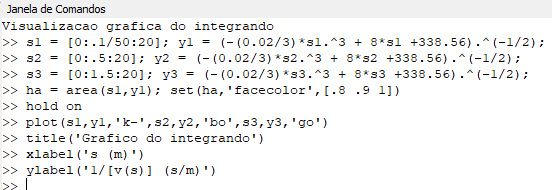
\includegraphics[scale=1]{img5.png}
		\caption{Construção do Gráfico 1}
	\end{figure}
	
	\section{Conclusões}
	
	Em primeiro lugar, é possível afirmar que uma análise minimamente razoável do problema proposto pôde ser executada,
	de modo que as formulações matemáticas puderam ir ao encontro dos princípios físicos envolvidos na dinâmica do problema,
	possibilitando a determinação de valores confiáveis para as grandezas solicitadas.
	
	Outrossim, a alternativa de análise numérica encontrada para solucionar a integral a que se chegou no contexto da 
	determinação do valor de tempo decorrido mostrou-se robusta e pôde, inclusive, confirmar a aproximação visual inicial.
	
	Por fim, não se pode deixar de destacar o papel primordial dos recursos computacionais oferecidos pelo software 
	\textit{Octave} nas construções e determinações realizadas. 	  
	
\end{document}



